\begin{surferPage}[Sextica Barth]{La Séxtica de Barth}
    Esta superficie de grado $6$ (séxtica) fue construida por Wolf Barth en 1996.
    Tiene un total de $65$ singularidades, siendo el máximo posible para una séxtica,
    un hecho demostrado poco tiempo después por Jaffe y Ruberman. Es decir,
    ¡el récord mundial de Barth es insuperable!

    Esta construcción de Barth fue una gran sorpresa, ya que por mucho tiempo
    se pensó que las superficies de grado $6$ sólo podían tener hasta $64$ singularidades.
    
    Una caracterísitica particular de la construcción es su simetría icosaedral;
    la figura muestra un icosaedro y sus planos simétricos:
  \begin{center}
      \vspace*{-0.1cm}
      \begin{tabular}{@{}c@{\ \ }c@{\,}c@{}}
        \begin{tabular}{@{}c}
          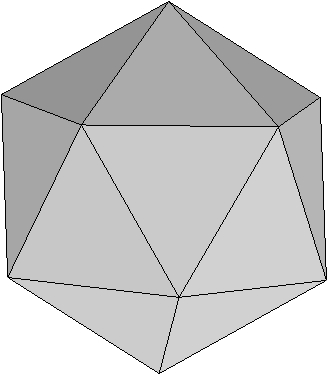
\includegraphics[width=1.4cm]{../../common/images/icosah}
        \end{tabular}
        &
        \begin{tabular}{@{}c}
          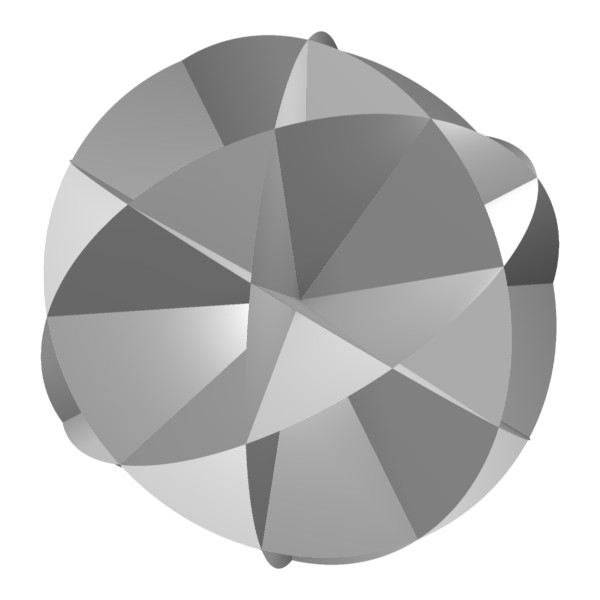
\includegraphics[width=1.4cm]{../../common/images/barth_sextic_planes}
        \end{tabular}
        &
        \begin{tabular}{c@{}}
          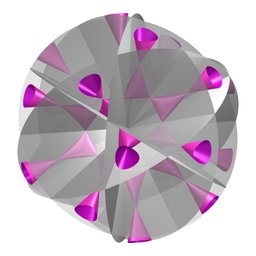
\includegraphics[width=1.4cm]{../../common/images/barth_sextic_and_planes}
        \end{tabular}
      \end{tabular}
    \end{center}
    \vspace*{-0.1cm}

    La séxtica de Barth satisface la ecuación
    $P_6 - \alpha K^2=0,$ donde $P_6$
    representa los seis planos simétricos,
    $K=x^2+y^2+z^2-1$ es la esfera unitaria y
    $\alpha=\frac{1}{4}(2+\sqrt{5})$.
\end{surferPage}
